\subsection{Formulating a Neural Network model for Continuous-Time Processes}

In the following discussion, we only worry about time-independent (sometimes also refered to as autonomous) systems, as those are more relevant for control, but most of those approaches generalize well to time-dependent systems as well. Time-Continuous Neural Networks model dynamical systems model the evolution of the hidden states (which we denote as $\bm{x}_t$ at a given time $t$) of a neural network by equations of the form: 

\begin{align}
    \frac{\partial \bm{x}_t}{\partial t} = D(\bm{x}_t, \bm{I}_t, \theta).
\end{align}
 
 Where $D$ denotes some kind of model function that estimates the time-derivative of $\bm{x}_t$. $D$ is a function of $\bm{x}_t$, which denotes the hidden state of the neuron, $\bm{I}_t$ which denotes the inputs of the neuron and a learnable parameter vector $\theta$. Updates of the (hidden) state $\bm{x}_t$ are the computed using some ODE solver which integrates $\frac{\partial \bm{x}_t}{\partial t}$ over some time-step $\Delta t$ to compute $\bm{x}_{t+\Delta t} = \int_t^{t+\Delta t} \frac{\partial \bm{x}_t}{\partial t} + \bm{x}_t$.
 
 
 \begin{align}
    D(\bm{x}_t, \bm{I}_t, \theta) =  f(\bm{I}_t, \theta).
\end{align}
 
 It is worth noting that in a supervised learning context, this formulation has the advantage of being able to represent irregularly sampled time-sequences. For the control applications we consider here, the sample-rate is imposed by the hardware of our robot and is likely regular. In the original formulation of Chen et al, neural ODEs are not recurrent but a natural extension to recurrent neural networks can be formulated as: \\

 \begin{align}
    D(\bm{x}_t, \bm{I}_t, \theta) =  f(\bm{x}_t, \bm{I}_t, \theta).
\end{align}
 
Where the flow $D$ is not only a function of the input $\bm{I}_t$ but also of the inner-state $\bm{x}_t$. Such a model can be though of as a recurrent neural network where the recurrent connection are implemented by an integrator.

\begin{figure}[h!]
    \centering
    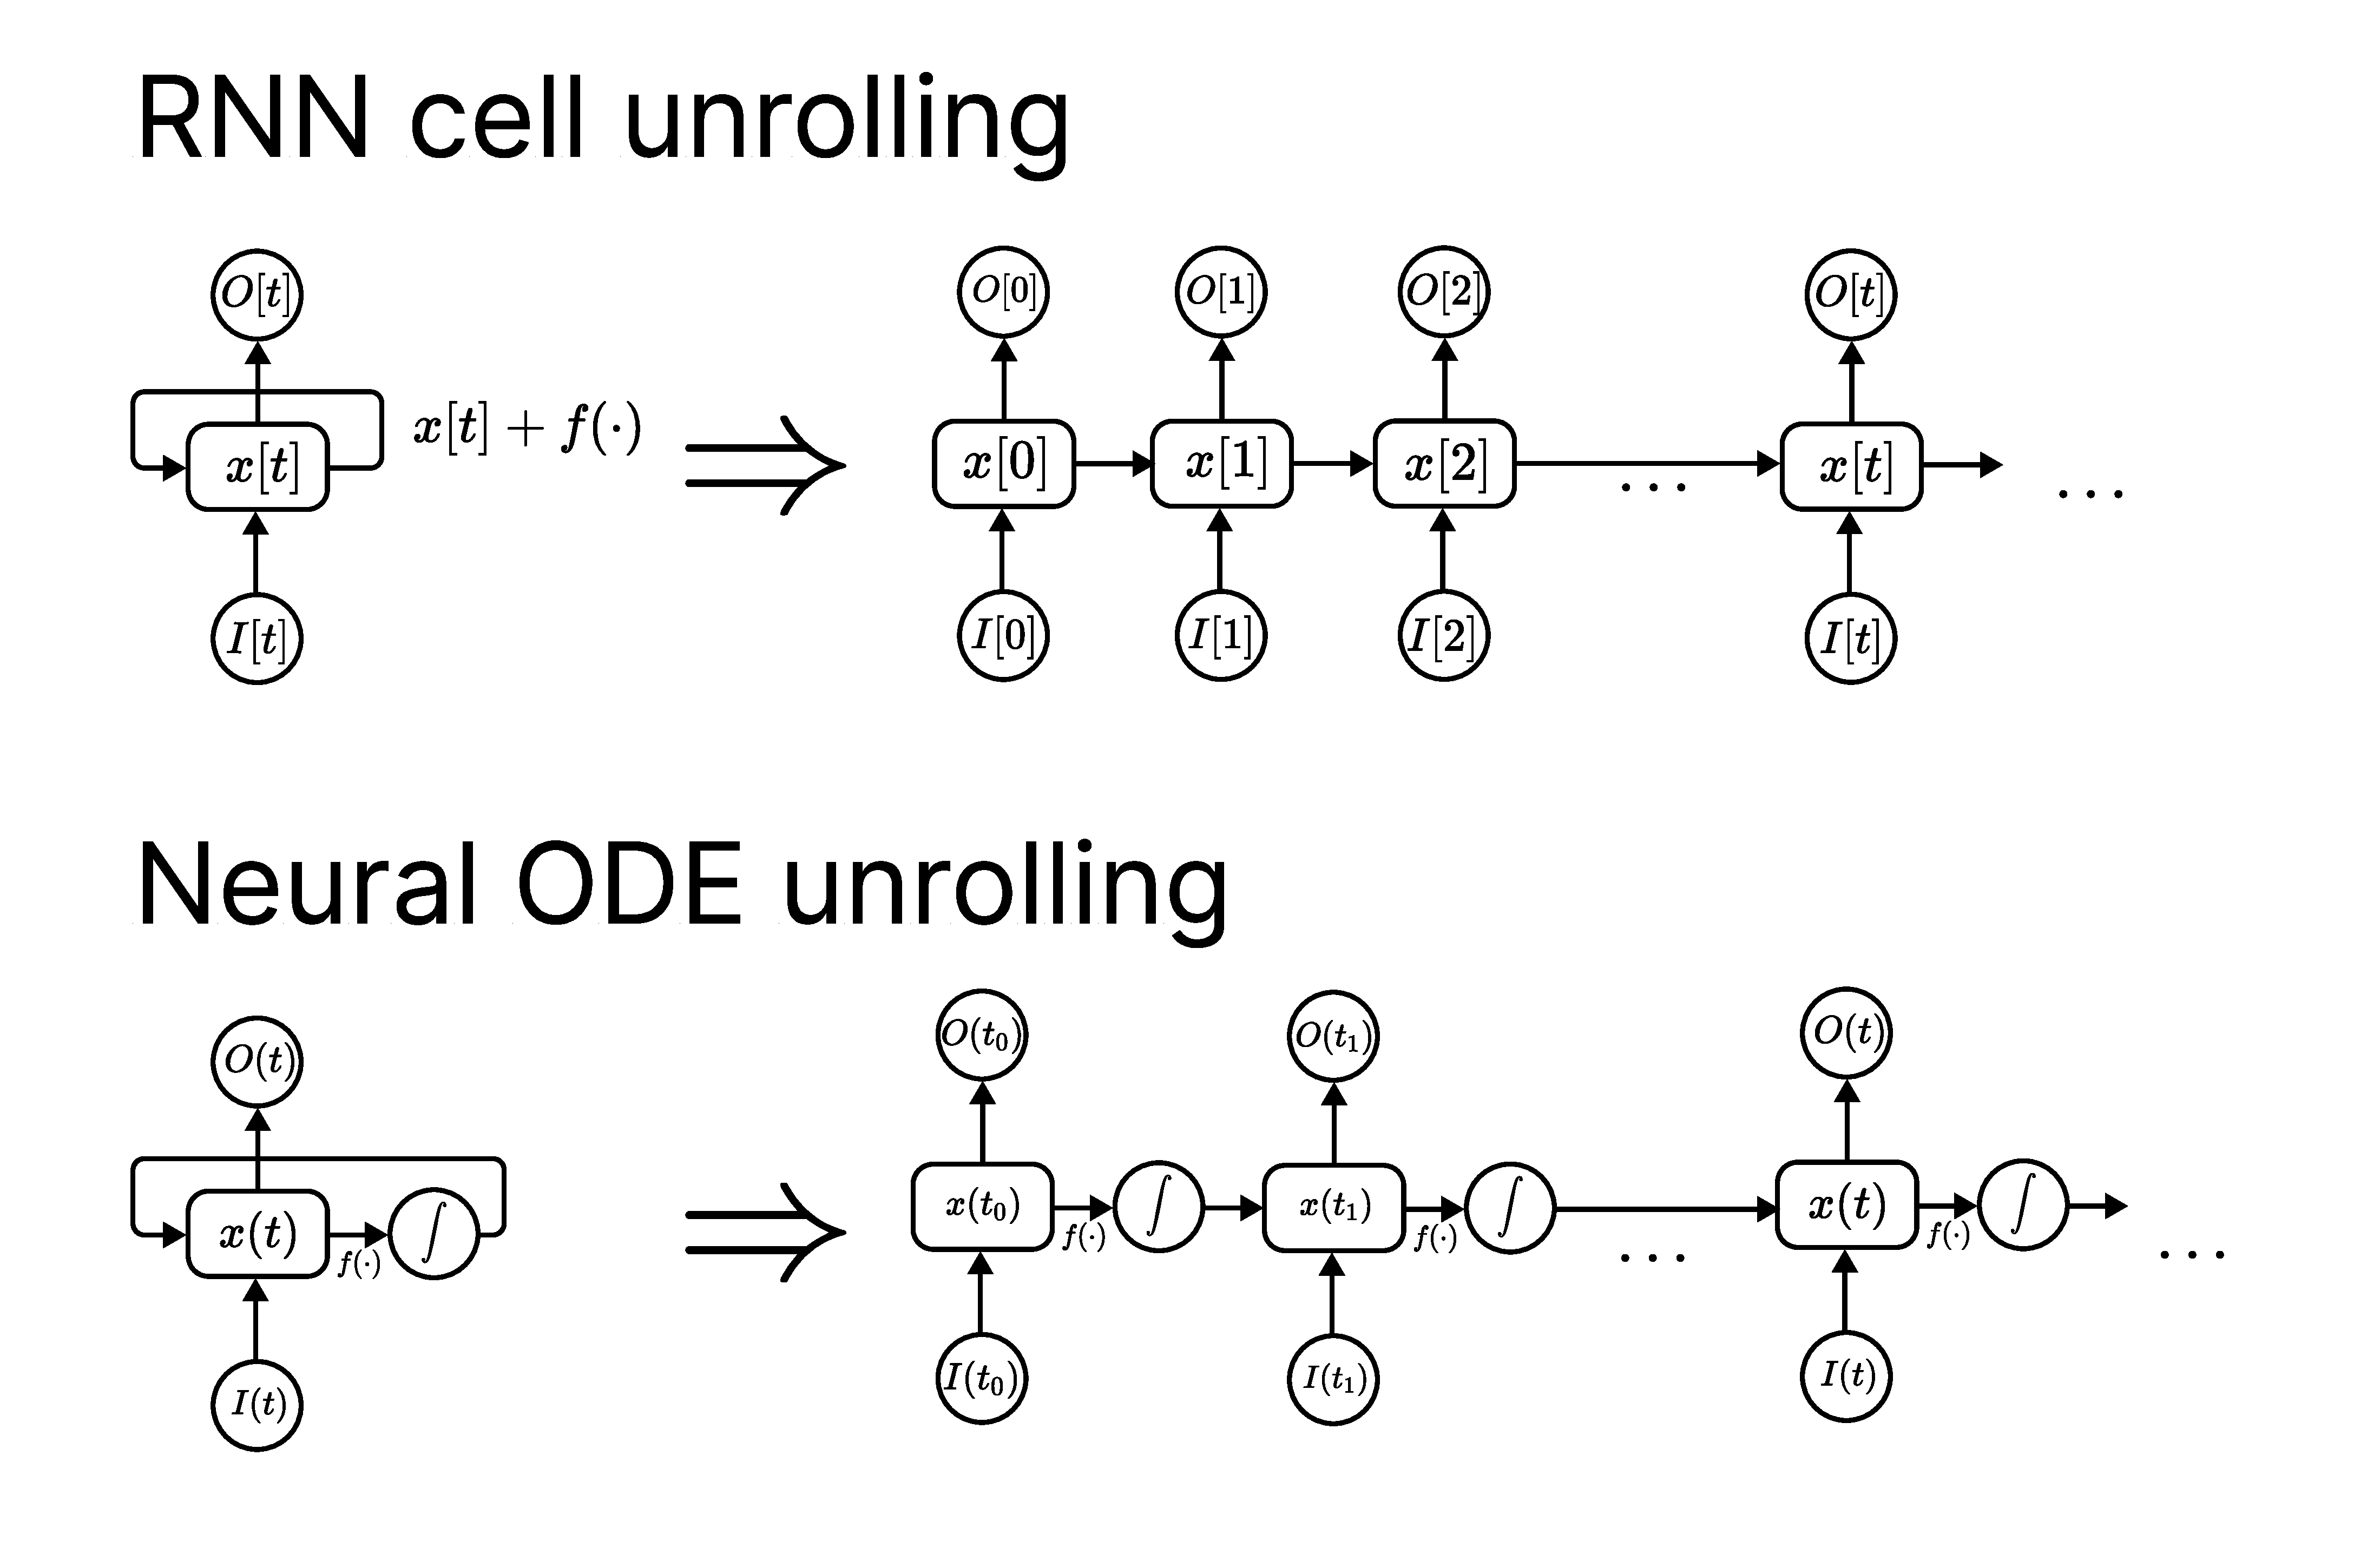
\includegraphics[width=0.45\textwidth]{figures/unroll.pdf}
    \caption{An illustration of the difference between Neural ODE unrolling v.s. RNN unrolling.}
\end{figure}

 The most straight forward approach to that problem is directly using a neural network to model the flow $D$, this is the approach chosen by \cite{Chen2018NeuralOD} (which is often referred to as "Neural-ODEs"). An alternative provided by an earlier contribution is the so called "Continuous-Time Recurrent Neural Network" model (CT-RNNs) first proposed by Funahashi and Nakamura in \cite{Funahashi1993ApproximationOD}, which pick $D$ as: 
 
\begin{align}
    D(\bm{x}_t, \bm{I}_t, \theta) = -\frac{\bm{x}_t}{\tau} + f(\bm{x}_t, \bm{I}_t, \theta).
\end{align}

where $\tau$ is a fixed time constant (according to our formalism it is an element of the vector $A$) and $f$ a non-linear activation function. The fixed time-constant is is introduced to induce a decay in the behavior of the neurons which is meant to enable recurrent connections which avoiding unstable neuron dynamics. In their original paper, Funahashi and Nakamura propose to use $f = \sum_{j=1}^m w_{i,j} \cdot \sigma\left( x_{i,t} \right) + I_i (t)$, where the weights $w{i,j}$ are elements of the vector $\theta$. \\

More recently, one suggested implementation that seems to give better performance is proposed by Hasani and Lechner though so-called "Liquid Time-Constant networks (LTCs)" \cite{Hasani2021LiquidTN}. In that case the activation $f$ affects both the time-constant and the non-linearity (hence make the time-constant "liquid"), this approach corresponds to the following time-derivative model:

\begin{align}
    D(\bm{x}_t, \bm{I}_t, \theta) = - \left[ \frac{1}{\tau} + A f(\bm{x}_t, \bm{I}_t, \theta, A) \right] \bm{x}_t \nonumber \\ + f(\bm{x}_t, \bm{I}_t, \theta).
\end{align}

Where $A$ is a so called \textit{bias} parameter which con-trolls the non-linearity in the synaptic response. In practice, Hasani and Lechner propose to use the following activation function: $f(\bm{x}_t, \bm{I}_t, \theta, A) = \tanh (w^\textit{inner} \bm{x} + w^\textit{inputs} \bm{I} + \mu)$, which is loosely connected to the non-linearity observed in synaptic dynamics between biological neurons \cite{Lechner2020NeuralCP}.

\begin{table}[h!]
\centering
\caption{Time-Continuous Neural Network Classes}
\resizebox{\columnwidth}{!}{%
\begin{tabular}{l|c|c}
\textbf{ } & \textbf{Hidden state equation} & \textbf{ Recurrent? } \\ 
\hline
CT-RNN & $ \frac{\partial \bm{x}_t}{\partial t} = -\frac{\bm{x}_t}{\tau} + f(\bm{x}_t, \bm{I}_t, \theta)$ & Yes \\
LTC & $ \frac{\partial \bm{x}_t}{\partial t} = - \left[ \frac{1}{\tau} + f(\bm{x}_t, \bm{I}_t, \theta) \right] \bm{x}_t + f(\bm{x}_t, \bm{I}_t, \theta)$ & Yes \\
Neural-ODE &  $ \frac{\partial \bm{x}_t}{\partial t} = f(\bm{x}_t, \bm{I}_t, \theta)$ & No \\
RNN-ODE &  $ \frac{\partial \bm{x}_t}{\partial t} = f(\bm{x}_t, \bm{I}_t, \theta)$ & Yes
\end{tabular}%
}
\end{table}


\subsection{Training}

Compared to multi-layer perceptrons and RNNs computing gradients on continuous time neural networks is way less obvious because of the integrator step. In the following section we discuss two approaches to the computation of such gradients together with their pros and cons. Two main approaches are possible \textit{backpropagation through time} (BPTT, which is recommanded by Hasani et al. \cite{Hasani2021LiquidTN}) and the \textit{adjoint sensitivity method} (which is recommended by Chen et al \cite{Chen2018NeuralOD}). \\

\textit{Backpropagation through time} works by directly computed the gradient of a loss function through the ODE solver (it requires our ODE solver to build a computation graph and then we use \textit{autograd} to compute a gradient). \\
\textbf{TODO: Finish write up on BPTT}
\\
The \textit{adjoint sensitivity method} required saving a so-called adjoint state $\bm{a}(t) = \frac{\partial L}{\partial \bm{z}(t)}$ throughout the unrolling of the neural network.

\textbf{TODO: Finish write up on the adjoint method}

\subsection{Continuous Time Neural Network Cells}
\label{sec:nn_cell}

\begin{figure}[h!]
    \centering
    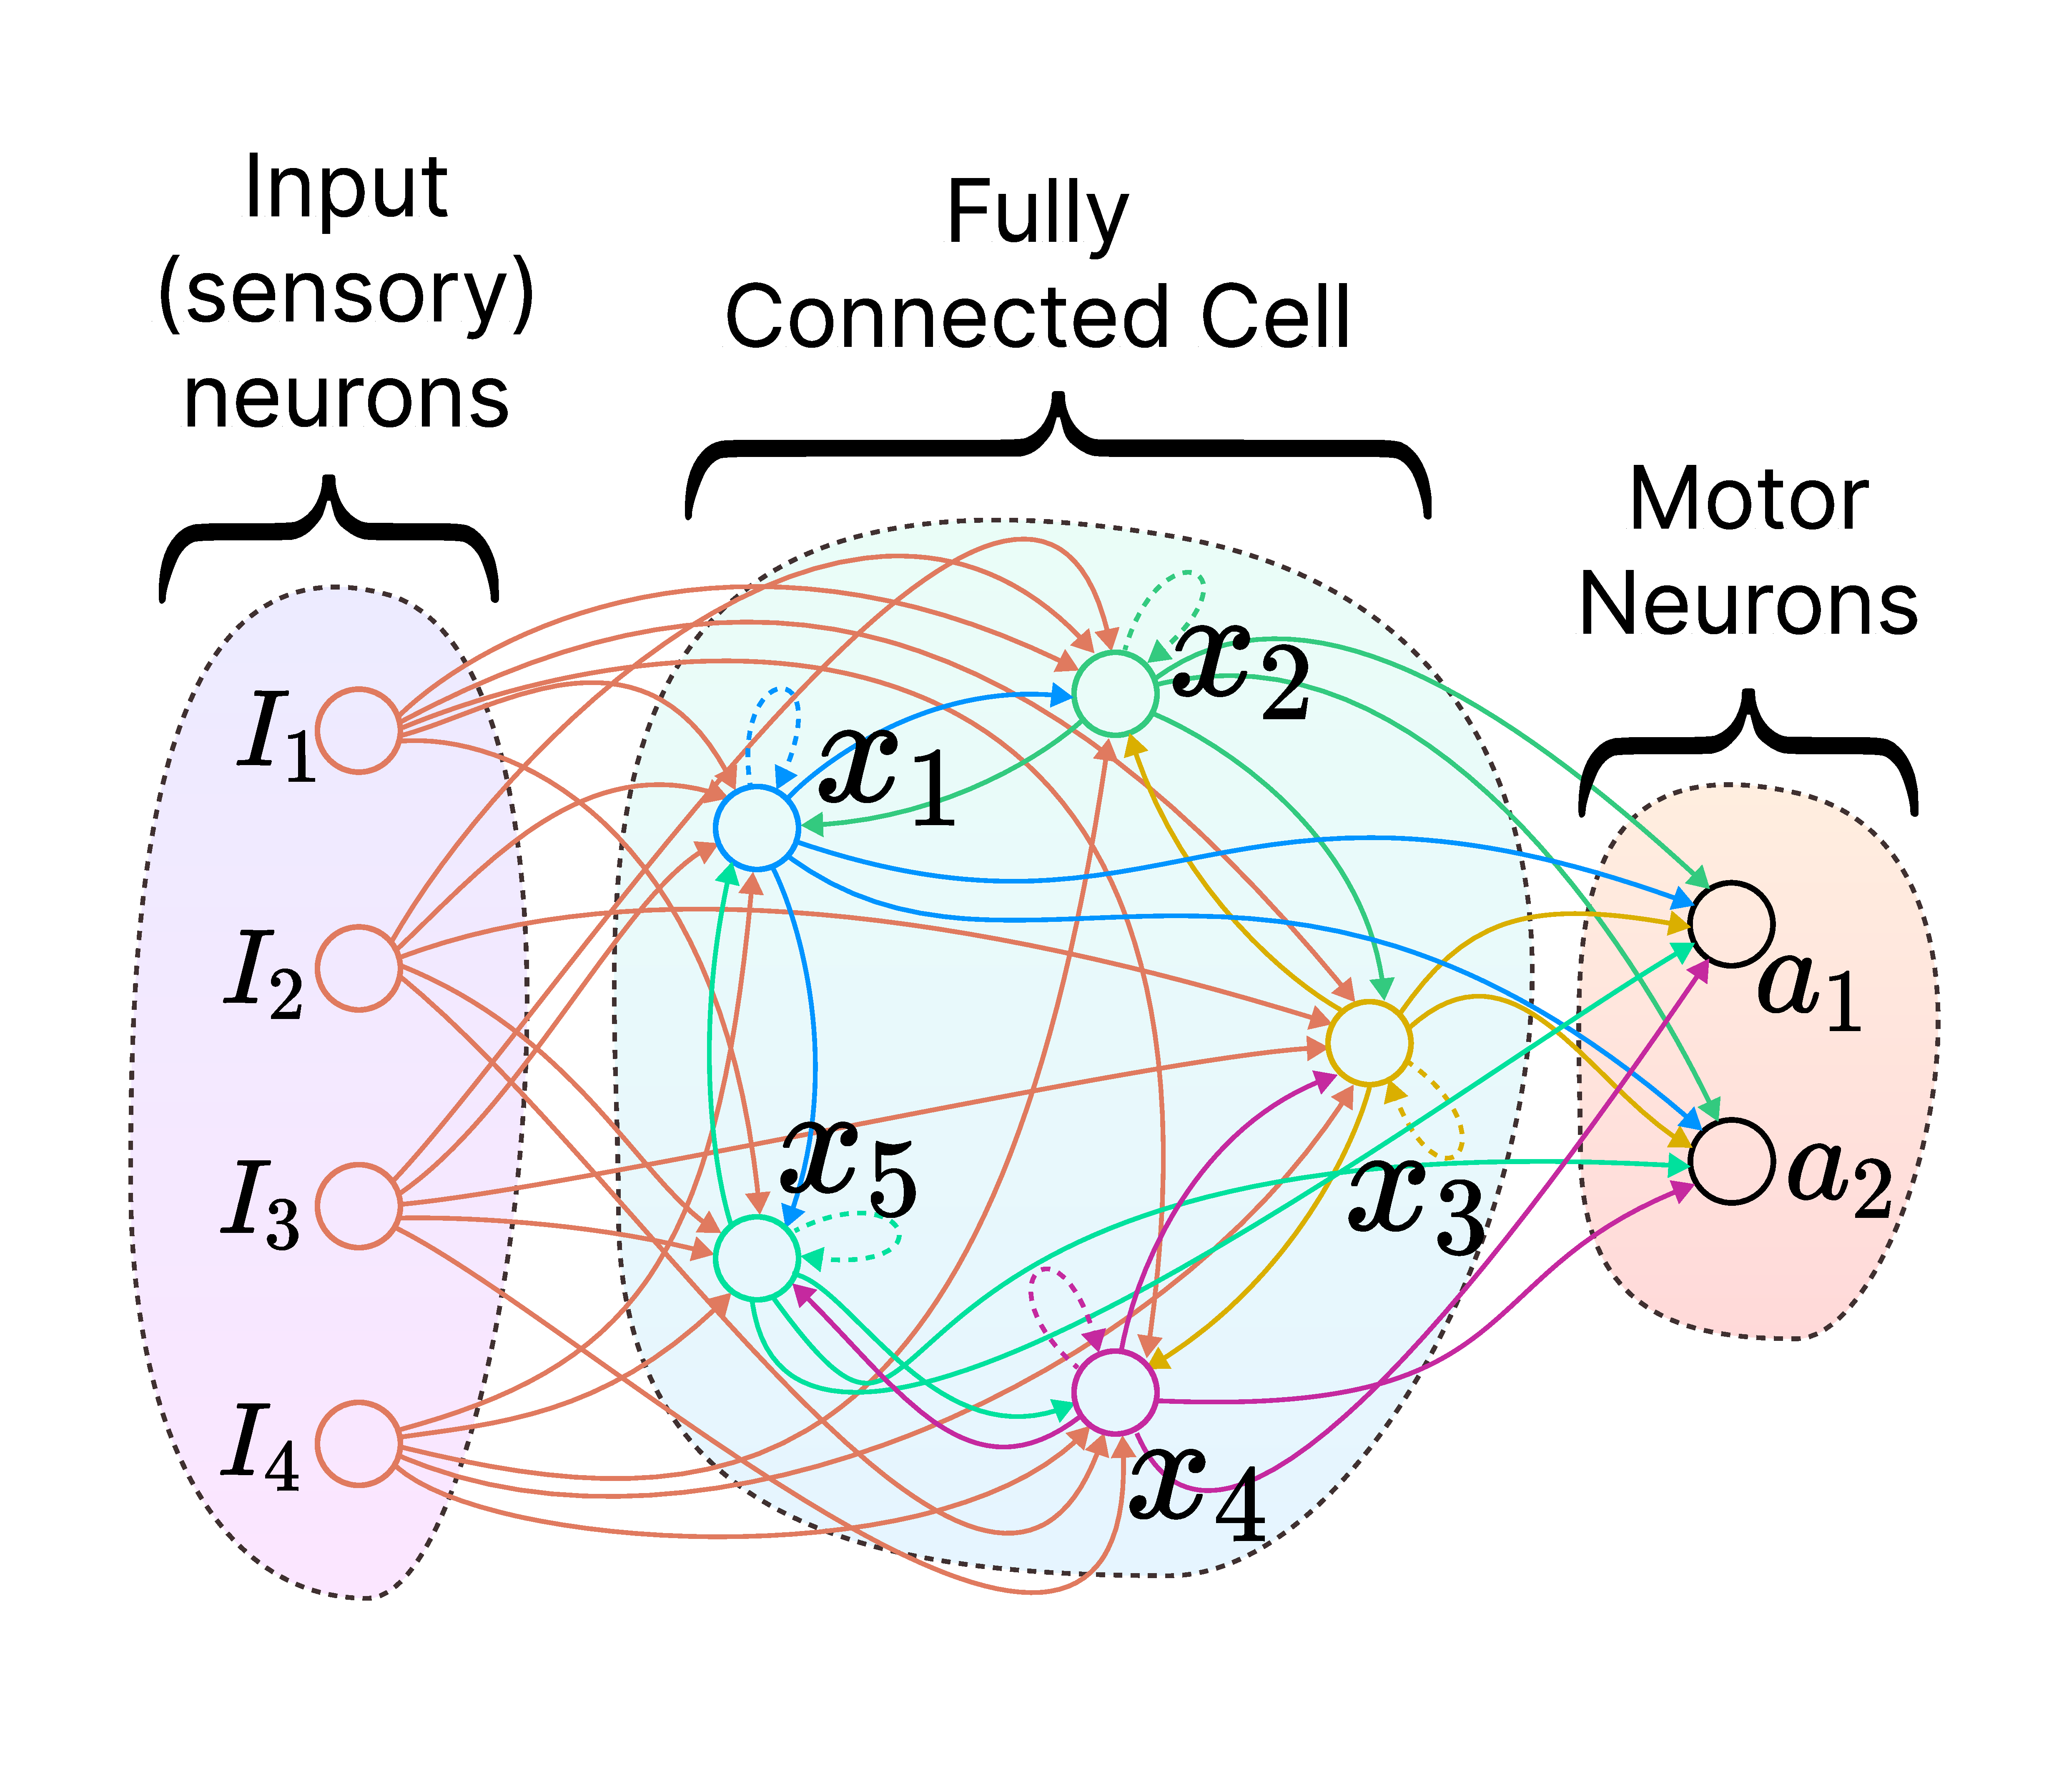
\includegraphics[width=0.45\textwidth]{figures/LTC_Cell.pdf}
    \caption{Fully connected Time-Continuous Neural Network Cell. With 4 inputs ($o_{1,\dots,4}$), 5 inner-neurons (with inner states $x_{1,\dots,5}$) and 2 motor neurons (outputs $I_{1,2}$).}
    \label{fig:cell_drawing}
\end{figure}

In order to deal with the motor task that we consider in this project we choose to investigate small fully connected neuron cells that take a $n$-dimensional input, contain $k$ inner-neurons and return $d$ outputs (we call the outputs "\textit{motor neurons}") We provide a visual representation of such a cell in figure \ref{fig:cell_drawing}. Most of our experiments are performed with LTC cells, so we will explicitly derive the forward pass equations for an LTC, but we can build equivalent cells for RNN-ODE and CT-RNN cells in a very similar fashion.\\

For a given inner-neuron $i$, the flow of it's state is computed according to the following equation: 

\begin{footnotesize}
    \begin{align*}
        \frac{dx_i}{dt} = f_i(\textbf{x},\textbf{I},\theta)\\
        = - \frac{x_i}{\tau_i} +
        \tanh \left( \sum_{j=1}^{n} w_{ij}^\textit{inputs} I_j +\sum_{j=1}^{n} w_{ij}^\textit{inner} x_j  +\mu_i\right) (A_i-x_i).
    \end{align*}
\end{footnotesize}

The states of each neurons are then passed through a linear layer to compute the output values as follows. Each output value's is computed as:

\begin{align*}
    o_i =  \sum_{j=1}^{k} w_{ij}^\textit{output} x_j 
\end{align*}

Note that this implies that each neuron's flow is influenced by it's input, every single other neuron on the same layer and also itself (it has a recurrent connection). This gives $k\cdot(k+n+d)$ connections in a single LTC cell, which is much denser than a typical multi-layer perceptron. To take a concrete example, in the implementation section when we discuss a $16$ neuron LTC cell for solving the cart-pole problem, it has $352$ connections for $16$ neurons, where a $16$ neuron perceptron with a single hidden-layer perceptron would only have $96$.
% \subsubsection{Key questions to answer about TCNs}
% \begin{itemize}
%     \item Network properties
%     \begin{itemize}
%         \item Why use CT-RNNs instead of RNNs
%         \item Why use LTCs instead of CT-RNNs
%         \item What is the difference with Neural ODEs
%     \end{itemize}
%     \item Forward passes
%     \begin{itemize}
%         \item What solver to used for the ODE step
%     \end{itemize}
%     \item Training
%     \begin{itemize}
%         \item How does BPTT works?
%     \end{itemize}
% \end{itemize}